
\documentclass[8pt]{article}

\usepackage[utf8]{inputenc}

\usepackage{amsmath, bm}
\usepackage{graphicx}
\usepackage{amssymb}
\usepackage{float}
\usepackage{caption}
\usepackage{subcaption}
% set font size to 11pt

% set margin
\usepackage[margin=1in]{geometry}

\setlength{\parskip}{\baselineskip}%
\setlength{\parindent}{0pt}%
\setlength{\headsep}{5pt}

\begin{document}

% insert pdf cover page here


\title{Experimental Propeller Performance}
\author{lwp26}
\date{October 2024}
\maketitle

\section{Introduction}

A simple experimental setup was made to collect thrust and power data for different propeller designs.
The acoustic spectrum of the propellers was also crudely measured to identify sources of noise 


\section{Method}

The setup consisted of a automatically calibrating load cell, motor driver and microphone.
The microphone was connected to a picoscope to measure the spectrum of the noise generated by the propellers.

The motor is ramped up in a staircase function where thrust and power are measured before the new step to allow time to settle.
At the beginning of each run the thrust is automatically calibrated by automatically applying and releasing a known weight.

The microphones position is very important as the noise generated close to the propeller was observed to be very directional.
The far field noise could not be measured due to lack of sensitivity and presence of background noise.

Noise measurements were also poor due to poor acoustics with some reflective surfaces, (e.g. table) close to the propellers.


\begin{figure}
    \centering
    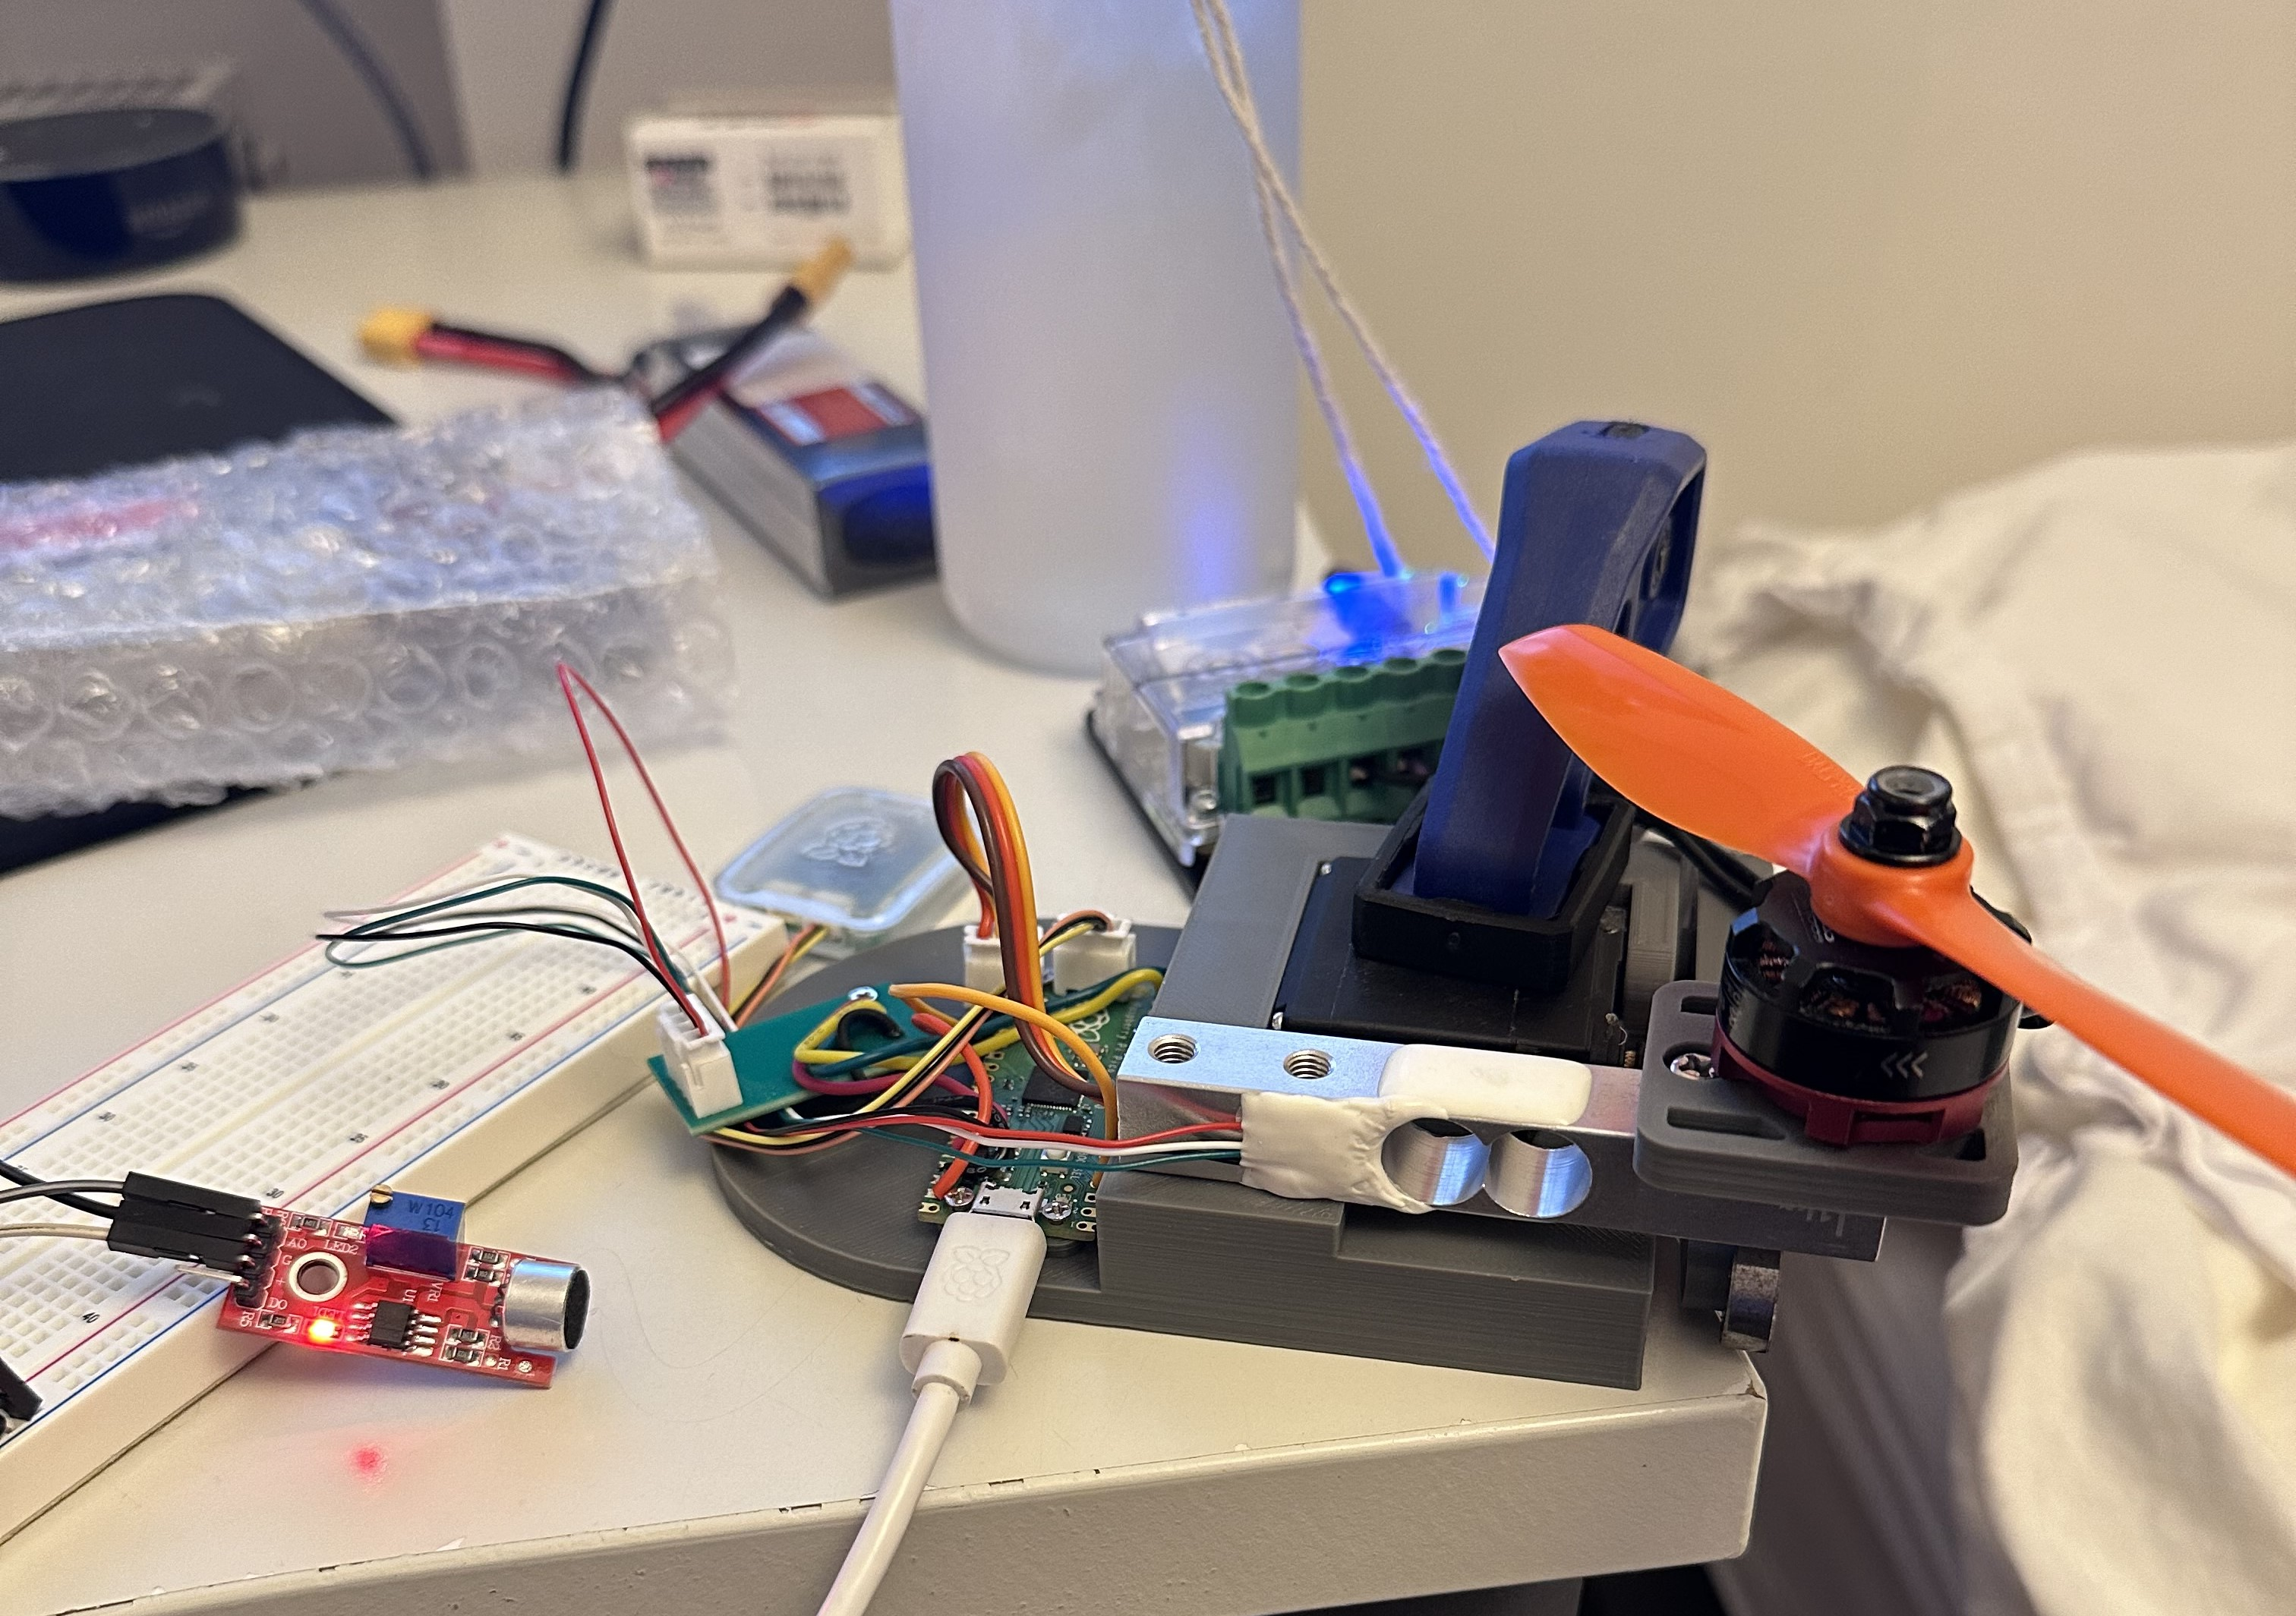
\includegraphics[width=0.99\textwidth]{setup.jpg}
    \caption{Experimental setup. The known mass was a 500ml water bottle.}
    \label{fig:setup}
\end{figure}

\section{Results}

\begin{figure}[H]
    \centering
    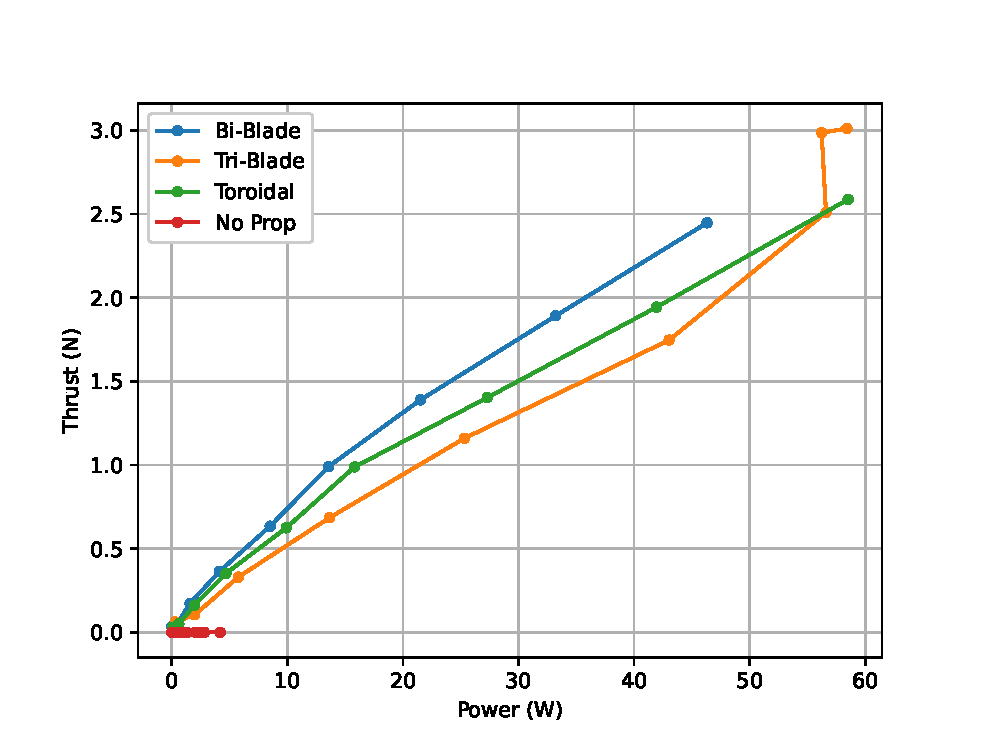
\includegraphics[width=0.99\textwidth]{power_vs_thrust.eps}
    \caption{Measured motor driver power vs measured thrust}
    \label{fig:power_vs_thrust}
\end{figure}

\begin{figure}[H]
    \centering
    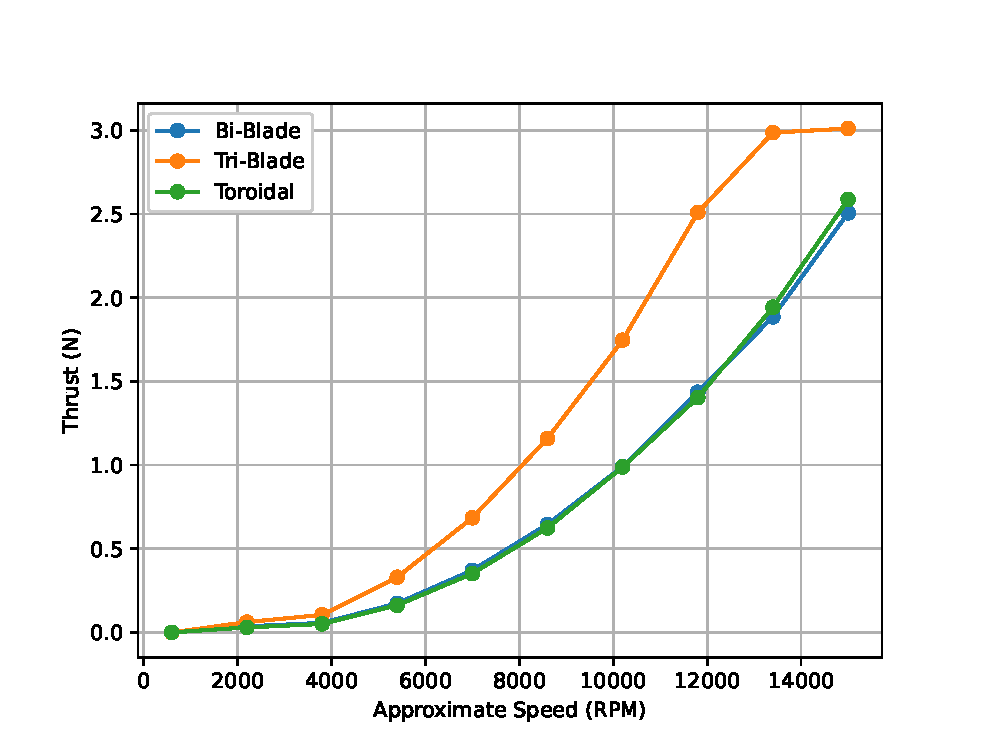
\includegraphics[width=0.99\textwidth]{speed_vs_thrust.eps}
    \caption{Measured motor driver power vs measured thrust}
    \label{fig:speed_vs_thrust}
\end{figure}

\begin{figure}[H]
    % subfigure
    \begin{subfigure}{0.99\textwidth}
        \centering
        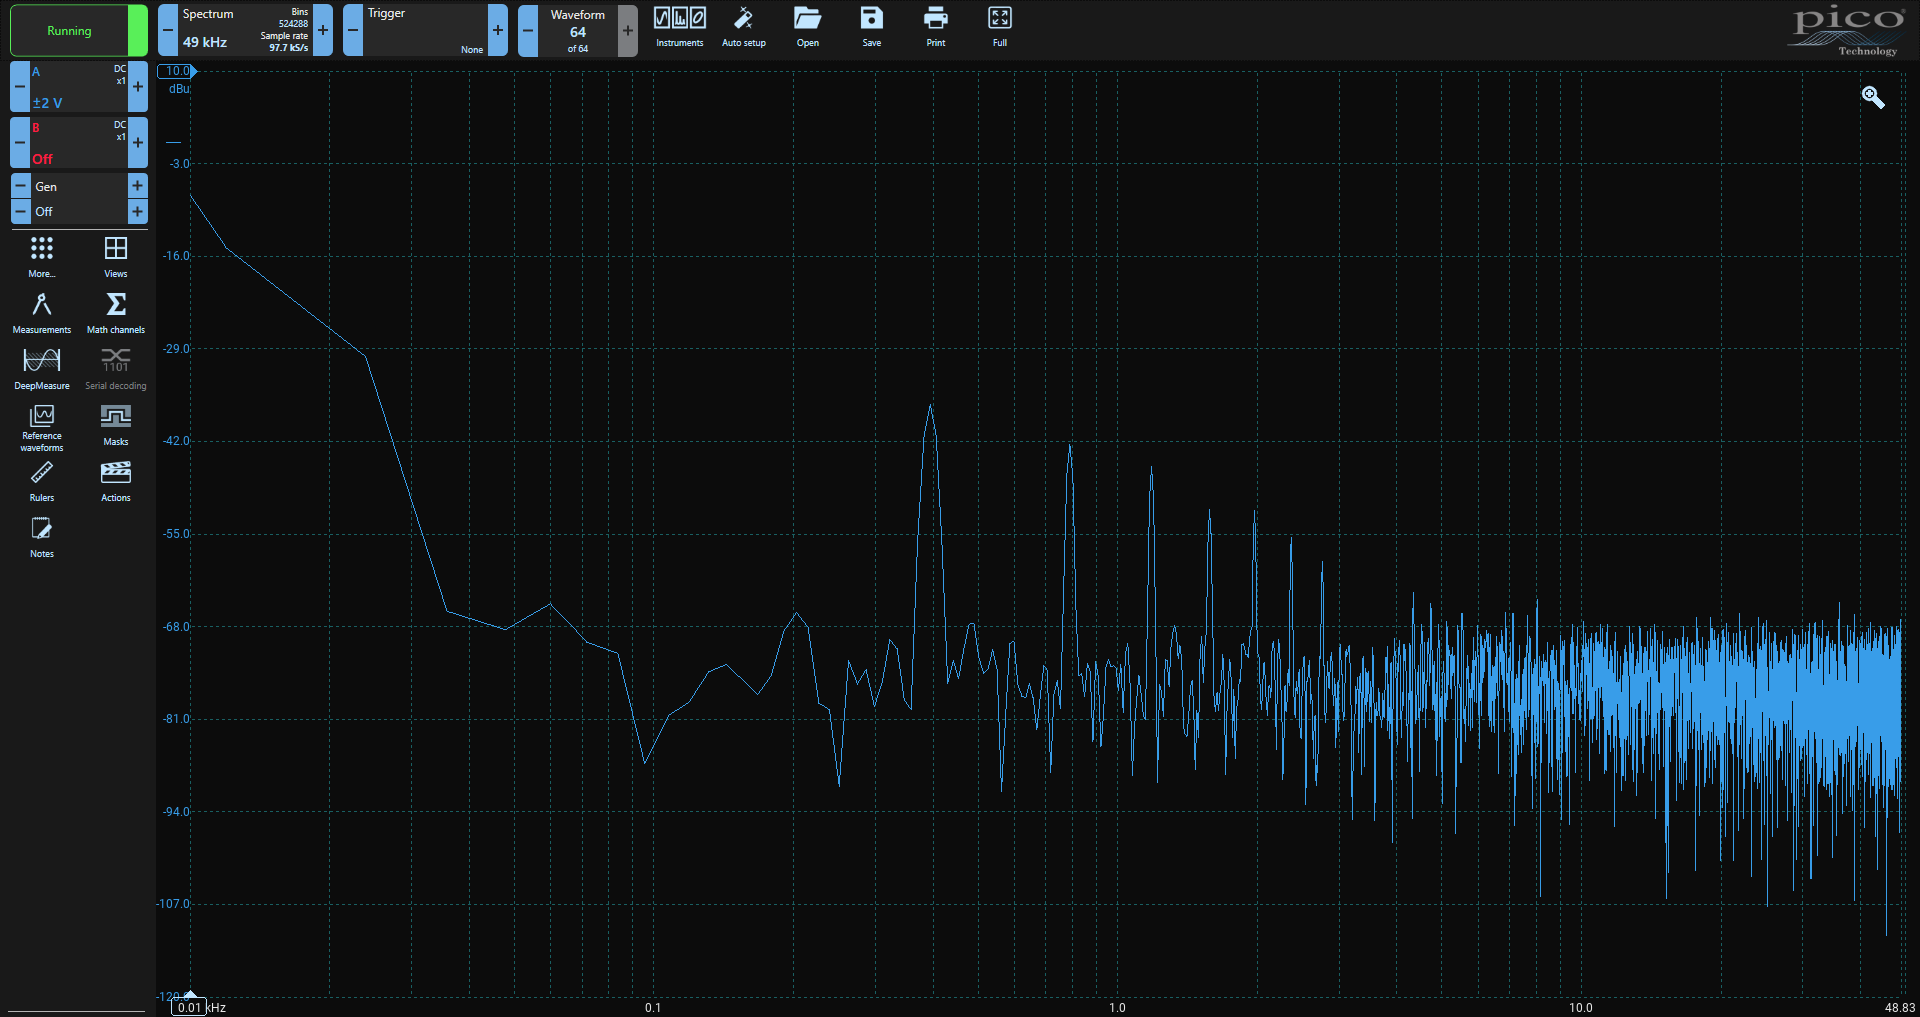
\includegraphics[width=0.99\textwidth]{hispeed_biprop.png}
        \caption{Bi-Propeller}
        \label{fig:hispeed_biprop}
    \end{subfigure}
    % subfigure
    \begin{subfigure}{0.99\textwidth}
        \centering
        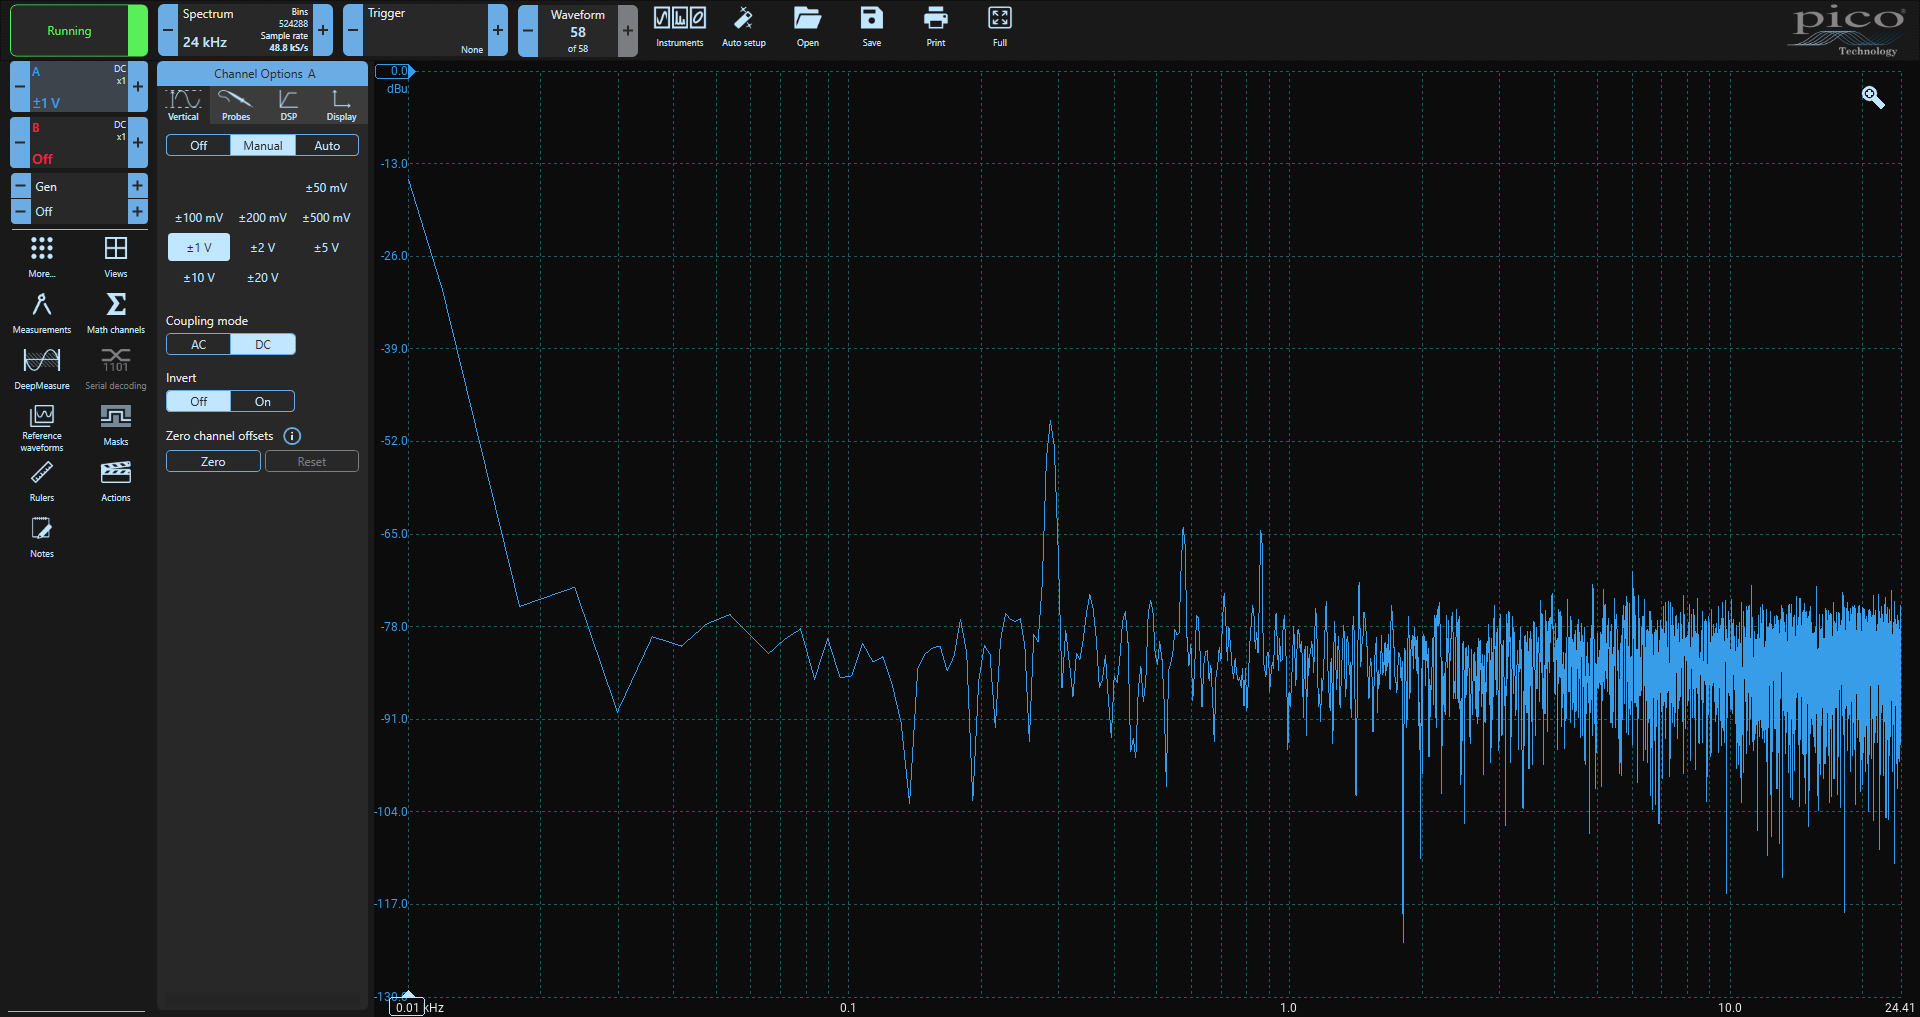
\includegraphics[width=0.99\textwidth]{hispeed_toroid.png}
        \caption{Toroidal propeller}
        \label{fig:hispeed_toroid}
    \end{subfigure}
    \caption{Noise spectrum of propellers at high speed}
    \label{fig:noise_spectrum_hispeed}
\end{figure}

\begin{figure}[H]
    % subfigure
    \begin{subfigure}{0.99\textwidth}
        \centering
        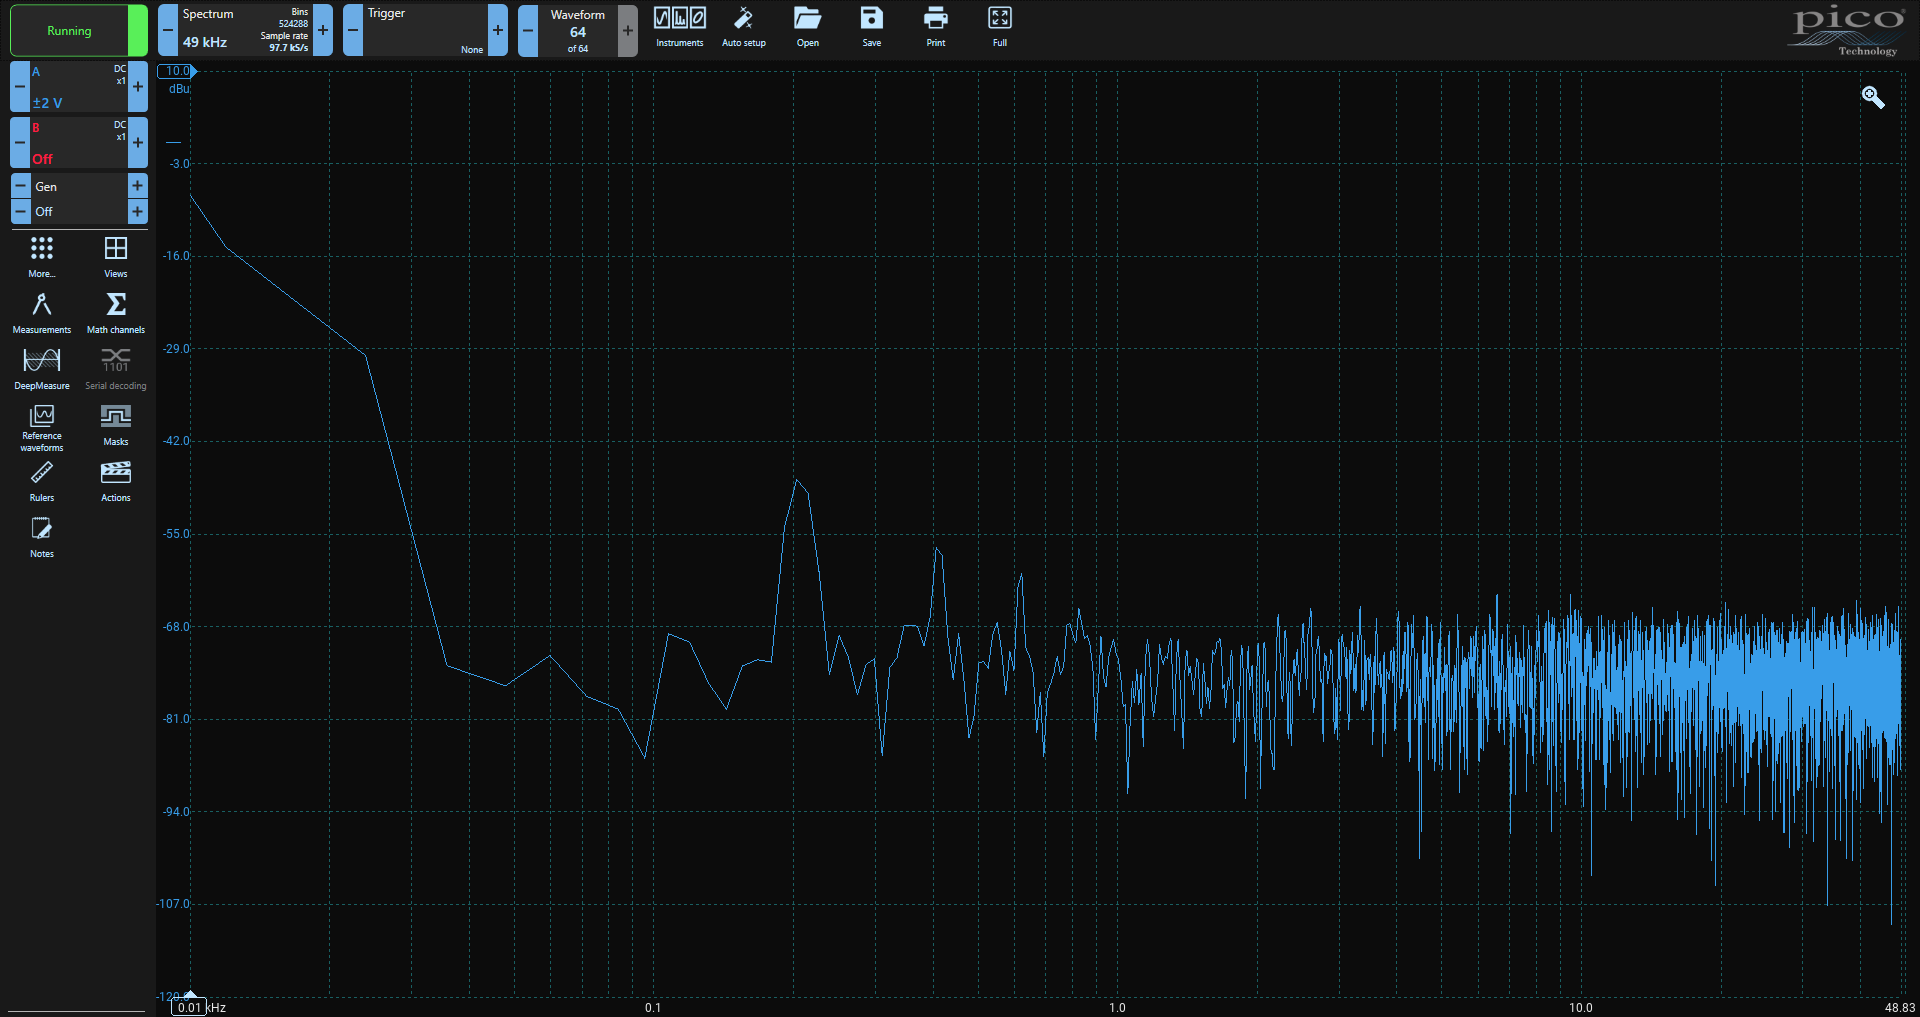
\includegraphics[width=0.99\textwidth]{lospeed_biprop.png}
        \caption{Bi-Propeller}
        \label{fig:lospeed_biprop}
    \end{subfigure}
    % subfigure
    \begin{subfigure}{0.99\textwidth}
        \centering
        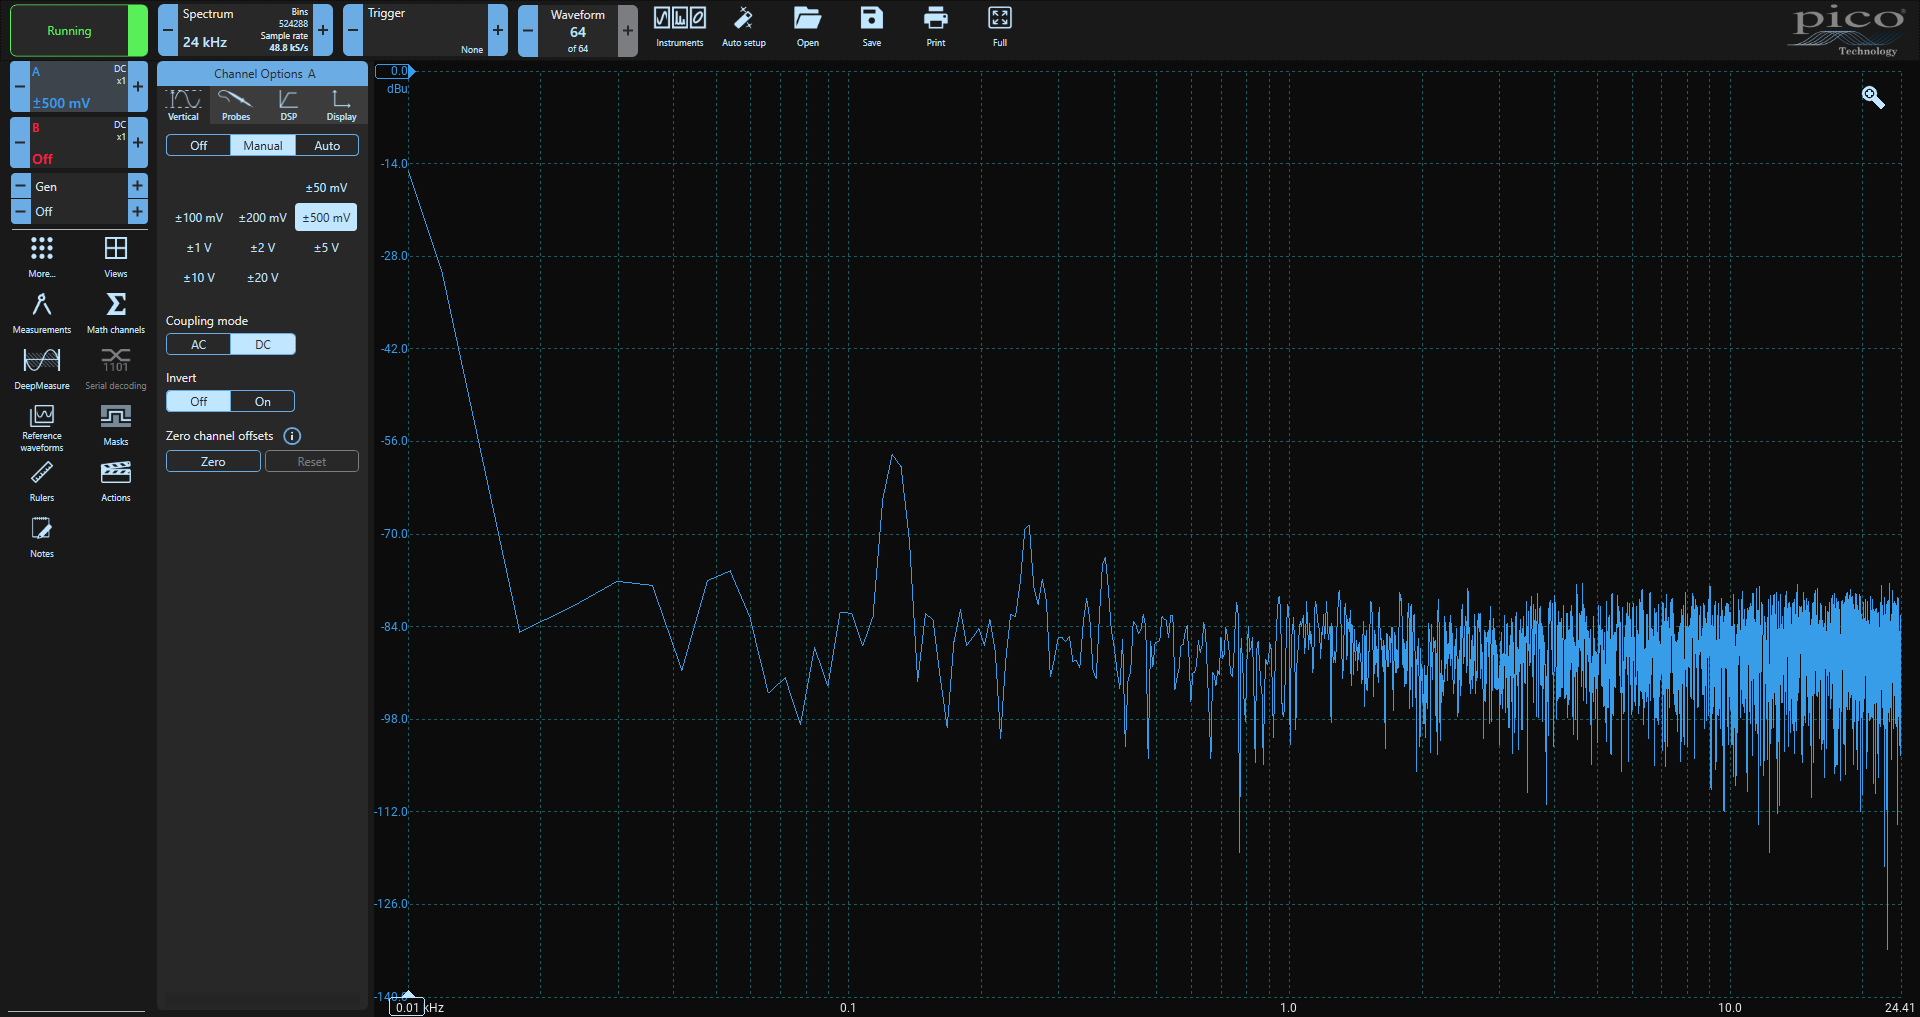
\includegraphics[width=0.99\textwidth]{lospeed_toroid.png}
        \caption{Toroidal propeller}
        \label{fig:lospeed_toroid}
    \end{subfigure}
    \caption{Noise spectrum of propellers at low speed}
    \label{fig:noise_spectrum_lospeed}
\end{figure}

\section{Discussion}



\section{Conclusion}

\end{document}
